\documentclass{article}\usepackage[]{graphicx}\usepackage[]{color}
%% maxwidth is the original width if it is less than linewidth
%% otherwise use linewidth (to make sure the graphics do not exceed the margin)
\makeatletter
\def\maxwidth{ %
  \ifdim\Gin@nat@width>\linewidth
    \linewidth
  \else
    \Gin@nat@width
  \fi
}
\makeatother

\definecolor{fgcolor}{rgb}{0.345, 0.345, 0.345}
\newcommand{\hlnum}[1]{\textcolor[rgb]{0.686,0.059,0.569}{#1}}%
\newcommand{\hlstr}[1]{\textcolor[rgb]{0.192,0.494,0.8}{#1}}%
\newcommand{\hlcom}[1]{\textcolor[rgb]{0.678,0.584,0.686}{\textit{#1}}}%
\newcommand{\hlopt}[1]{\textcolor[rgb]{0,0,0}{#1}}%
\newcommand{\hlstd}[1]{\textcolor[rgb]{0.345,0.345,0.345}{#1}}%
\newcommand{\hlkwa}[1]{\textcolor[rgb]{0.161,0.373,0.58}{\textbf{#1}}}%
\newcommand{\hlkwb}[1]{\textcolor[rgb]{0.69,0.353,0.396}{#1}}%
\newcommand{\hlkwc}[1]{\textcolor[rgb]{0.333,0.667,0.333}{#1}}%
\newcommand{\hlkwd}[1]{\textcolor[rgb]{0.737,0.353,0.396}{\textbf{#1}}}%

\usepackage{framed}
\makeatletter
\newenvironment{kframe}{%
 \def\at@end@of@kframe{}%
 \ifinner\ifhmode%
  \def\at@end@of@kframe{\end{minipage}}%
  \begin{minipage}{\columnwidth}%
 \fi\fi%
 \def\FrameCommand##1{\hskip\@totalleftmargin \hskip-\fboxsep
 \colorbox{shadecolor}{##1}\hskip-\fboxsep
     % There is no \\@totalrightmargin, so:
     \hskip-\linewidth \hskip-\@totalleftmargin \hskip\columnwidth}%
 \MakeFramed {\advance\hsize-\width
   \@totalleftmargin\z@ \linewidth\hsize
   \@setminipage}}%
 {\par\unskip\endMakeFramed%
 \at@end@of@kframe}
\makeatother

\definecolor{shadecolor}{rgb}{.97, .97, .97}
\definecolor{messagecolor}{rgb}{0, 0, 0}
\definecolor{warningcolor}{rgb}{1, 0, 1}
\definecolor{errorcolor}{rgb}{1, 0, 0}
\newenvironment{knitrout}{}{} % an empty environment to be redefined in TeX

\usepackage{alltt}

\usepackage{amsmath, amssymb}
\usepackage{graphicx}
\usepackage{hyperref}
\IfFileExists{upquote.sty}{\usepackage{upquote}}{}
\begin{document}

\title{Pol Sci 630:  Problem Set 10 Solutions: 2SLS, Matching, Outlier, Heckman}

\author{Prepared by: Anh Le (\href{mailto:anh.le@duke.edu}{anh.le@duke.edu})}

\date{Due Date: Friday, Nov 6, 2015, 12 AM (Beginning of Lab)}

\maketitle

\section{2SLS}

\textbf{\color{red} Insert your comments on the assignment that you are grading above the solution in bold and red text. For example write: "GRADER COMMENT: everything is correct! - 8/8 Points" Also briefly point out which, if any, problems were not solved correctly and what the mistake was. See below for more examples.}

\subsection{Load dataset CigarettesSW from package AER}

\begin{knitrout}
\definecolor{shadecolor}{rgb}{0.969, 0.969, 0.969}\color{fgcolor}\begin{kframe}
\begin{alltt}
\hlkwd{library}\hlstd{(AER)}
\hlkwd{data}\hlstd{(}\hlstr{"CigarettesSW"}\hlstd{)}
\end{alltt}
\end{kframe}
\end{knitrout}

\subsection{Plot the following}

What can we say about the relationship between tax, price, and packs? Note: This is a good way to show the relationship between 3 variables with a 2D plot.

\begin{knitrout}
\definecolor{shadecolor}{rgb}{0.969, 0.969, 0.969}\color{fgcolor}
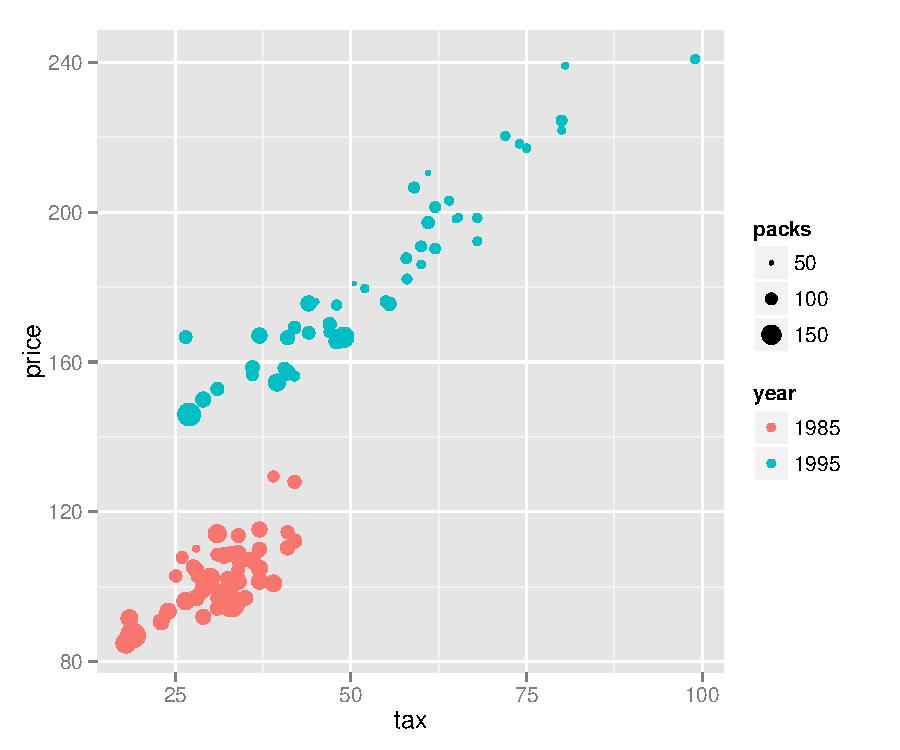
\includegraphics[width=\maxwidth]{figure/unnamed-chunk-2-1} 

\end{knitrout}

\textbf{Solution}

Tax and price are positively correlated. This gives a hint that tax can be a good instrument for price.

Tax and price are negatively correlated with the number of cigarette packs consumed per capita.

\subsection{Divide variable income by 1000 (for interpretability)}

\begin{knitrout}
\definecolor{shadecolor}{rgb}{0.969, 0.969, 0.969}\color{fgcolor}\begin{kframe}
\begin{alltt}
\hlstd{CigarettesSW}\hlopt{$}\hlstd{income} \hlkwb{<-} \hlstd{CigarettesSW}\hlopt{$}\hlstd{income} \hlopt{/} \hlnum{1000}
\end{alltt}
\end{kframe}
\end{knitrout}


\subsection{Run 2SLS}

Run 2SLS with \verb`ivreg`. Outcome: packs. Exogenous var: income. Endogenous var: price, whose instrument is tax. Interpret the coefficient of \verb`income` and \verb`price`.

\textbf{Solution}

\begin{kframe}
\begin{alltt}
\hlkwd{library}\hlstd{(stargazer)}
\hlstd{m11} \hlkwb{<-} \hlkwd{ivreg}\hlstd{(packs} \hlopt{~} \hlstd{income} \hlopt{+} \hlstd{price} \hlopt{|} \hlstd{income} \hlopt{+} \hlstd{tax,} \hlkwc{data} \hlstd{= CigarettesSW)}
\hlkwd{stargazer}\hlstd{(m11)}
\end{alltt}
\end{kframe}
% Table created by stargazer v.5.1 by Marek Hlavac, Harvard University. E-mail: hlavac at fas.harvard.edu
% Date and time: Fri, Oct 30, 2015 - 06:07:59 PM
\begin{table}[!htbp] \centering 
  \caption{} 
  \label{} 
\begin{tabular}{@{\extracolsep{5pt}}lc} 
\\[-1.8ex]\hline 
\hline \\[-1.8ex] 
 & \multicolumn{1}{c}{\textit{Dependent variable:}} \\ 
\cline{2-2} 
\\[-1.8ex] & packs \\ 
\hline \\[-1.8ex] 
 income & $-$0.00002 \\ 
  & (0.00002) \\ 
  & \\ 
 price & $-$0.398$^{***}$ \\ 
  & (0.055) \\ 
  & \\ 
 Constant & 168.488$^{***}$ \\ 
  & (7.673) \\ 
  & \\ 
\hline \\[-1.8ex] 
Observations & 96 \\ 
R$^{2}$ & 0.436 \\ 
Adjusted R$^{2}$ & 0.424 \\ 
Residual Std. Error & 19.637 (df = 93) \\ 
\hline 
\hline \\[-1.8ex] 
\textit{Note:}  & \multicolumn{1}{r}{$^{*}$p$<$0.1; $^{**}$p$<$0.05; $^{***}$p$<$0.01} \\ 
\end{tabular} 
\end{table} 


1000 dollar increase in income leads to \ensuremath{-2.2311969\times 10^{-5}} change in number of packs per capita, but the effect is not significant.

1 dollar increase in price leads to \ensuremath{-0.3978933} change in number of packs per capita, holding other constants. The coefficient is statistically significant.

\subsection{2SLS diagnostics: use F-test to check for weak instrument}

\textbf{Solution}

\begin{knitrout}
\definecolor{shadecolor}{rgb}{0.969, 0.969, 0.969}\color{fgcolor}\begin{kframe}
\begin{alltt}
\hlkwd{summary}\hlstd{(m11,} \hlkwc{diagnostics} \hlstd{=} \hlnum{TRUE}\hlstd{)}
\end{alltt}
\begin{verbatim}
## 
## Call:
## ivreg(formula = packs ~ income + price | income + tax, data = CigarettesSW)
## 
## Residuals:
##       Min        1Q    Median        3Q       Max 
## -56.16120 -10.40243   0.07866   6.87649  67.85671 
## 
## Coefficients:
##               Estimate Std. Error t value Pr(>|t|)    
## (Intercept)  1.685e+02  7.673e+00  21.957  < 2e-16 ***
## income      -2.231e-05  1.803e-05  -1.238    0.219    
## price       -3.979e-01  5.502e-02  -7.232 1.31e-10 ***
## 
## Diagnostic tests:
##                  df1 df2 statistic p-value    
## Weak instruments   1  93   341.145  <2e-16 ***
## Wu-Hausman         1  92     2.312   0.132    
## Sargan             0  NA        NA      NA    
## ---
## Signif. codes:  0 '***' 0.001 '**' 0.01 '*' 0.05 '.' 0.1 ' ' 1
## 
## Residual standard error: 19.64 on 93 degrees of freedom
## Multiple R-Squared: 0.436,	Adjusted R-squared: 0.4239 
## Wald test: 35.23 on 2 and 93 DF,  p-value: 4.081e-12
\end{verbatim}
\end{kframe}
\end{knitrout}

The weak instrument test (i.e. F-test) rejects the null hypothesis that the instrument is not correlated with the endogenous variable (p-value = \ensuremath{7.1137017\times 10^{-33}}). So our instruments are not weak.

\subsection{2SLS by hand}

Run the 2SLS by hand, i.e. not using \verb`ivreg`, but run 2 stages of \verb`lm`. Do you get the same estimate from \verb`ivreg`?

\textbf{Solution}

\begin{kframe}
\begin{alltt}
\hlstd{m_stage1} \hlkwb{<-} \hlkwd{lm}\hlstd{(price} \hlopt{~} \hlstd{tax,} \hlkwc{data} \hlstd{= CigarettesSW)}
\hlstd{CigarettesSW}\hlopt{$}\hlstd{price_hat} \hlkwb{<-} \hlkwd{predict}\hlstd{(m_stage1)}

\hlstd{m_stage2} \hlkwb{<-} \hlkwd{lm}\hlstd{(packs} \hlopt{~} \hlstd{income} \hlopt{+} \hlstd{price_hat,} \hlkwc{data} \hlstd{= CigarettesSW)}
\hlkwd{stargazer}\hlstd{(m_stage2)}
\end{alltt}
\end{kframe}
% Table created by stargazer v.5.1 by Marek Hlavac, Harvard University. E-mail: hlavac at fas.harvard.edu
% Date and time: Fri, Oct 30, 2015 - 06:07:59 PM
\begin{table}[!htbp] \centering 
  \caption{} 
  \label{} 
\begin{tabular}{@{\extracolsep{5pt}}lc} 
\\[-1.8ex]\hline 
\hline \\[-1.8ex] 
 & \multicolumn{1}{c}{\textit{Dependent variable:}} \\ 
\cline{2-2} 
\\[-1.8ex] & packs \\ 
\hline \\[-1.8ex] 
 income & $-$0.00003 \\ 
  & (0.00002) \\ 
  & \\ 
 price\_hat & $-$0.392$^{***}$ \\ 
  & (0.055) \\ 
  & \\ 
 Constant & 168.220$^{***}$ \\ 
  & (7.698) \\ 
  & \\ 
\hline \\[-1.8ex] 
Observations & 96 \\ 
R$^{2}$ & 0.427 \\ 
Adjusted R$^{2}$ & 0.415 \\ 
Residual Std. Error & 19.788 (df = 93) \\ 
F Statistic & 34.693$^{***}$ (df = 2; 93) \\ 
\hline 
\hline \\[-1.8ex] 
\textit{Note:}  & \multicolumn{1}{r}{$^{*}$p$<$0.1; $^{**}$p$<$0.05; $^{***}$p$<$0.01} \\ 
\end{tabular} 
\end{table} 


The coefficients are quite similar (by hand: \ensuremath{-0.3921355}, by ivreg: \ensuremath{-0.3978933})

\section{Matching}

\subsection{Load dataset lalonde from MatchIt, show covariate imbalance}

Plot the following. Hint: Look up \verb|position="dodge"| for ggplot2

\begin{knitrout}
\definecolor{shadecolor}{rgb}{0.969, 0.969, 0.969}\color{fgcolor}\begin{kframe}
\begin{alltt}
\hlkwd{library}\hlstd{(MatchIt)}
\end{alltt}


{\ttfamily\noindent\itshape\color{messagecolor}{\#\# Loading required package: MASS}}\begin{alltt}
\hlkwd{data}\hlstd{(}\hlstr{"lalonde"}\hlstd{)}
\hlkwd{ggplot}\hlstd{(}\hlkwc{data} \hlstd{= lalonde)} \hlopt{+}
  \hlkwd{geom_histogram}\hlstd{(}\hlkwd{aes}\hlstd{(}\hlkwc{x} \hlstd{= black,} \hlkwc{fill} \hlstd{=} \hlkwd{factor}\hlstd{(treat)),}
                 \hlkwc{position} \hlstd{=} \hlstr{"dodge"}\hlstd{)}
\end{alltt}


{\ttfamily\noindent\itshape\color{messagecolor}{\#\# stat\_bin: binwidth defaulted to range/30. Use 'binwidth = x' to adjust this.}}\end{kframe}
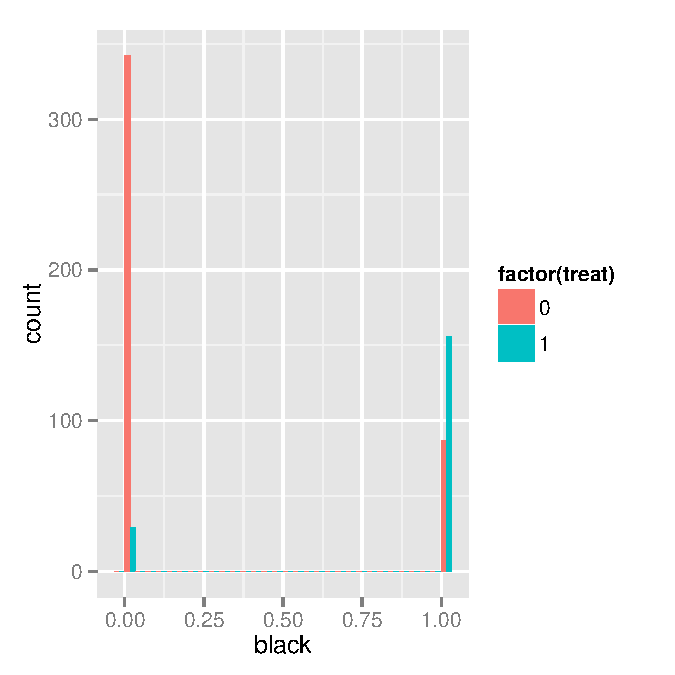
\includegraphics[width=\maxwidth]{figure/unnamed-chunk-7-1} 

\end{knitrout}

\subsection{See the effect of omitting an important variable}

Regress re78 against 1) treat, age, educ; 2) treat, age, educ, black. Do the treatment effect differ a lot? Why?

\textbf{Solution}

\begin{knitrout}
\definecolor{shadecolor}{rgb}{0.969, 0.969, 0.969}\color{fgcolor}\begin{kframe}
\begin{alltt}
\hlkwd{lm}\hlstd{(re78} \hlopt{~} \hlstd{treat} \hlopt{+} \hlstd{age} \hlopt{+} \hlstd{educ,} \hlkwc{data} \hlstd{= lalonde)}
\end{alltt}
\begin{verbatim}
## 
## Call:
## lm(formula = re78 ~ treat + age + educ, data = lalonde)
## 
## Coefficients:
## (Intercept)        treat          age         educ  
##     -851.74      -480.73        94.93       505.61
\end{verbatim}
\begin{alltt}
\hlkwd{lm}\hlstd{(re78} \hlopt{~} \hlstd{treat} \hlopt{+} \hlstd{age} \hlopt{+} \hlstd{educ} \hlopt{+} \hlstd{black,} \hlkwc{data} \hlstd{= lalonde)}
\end{alltt}
\begin{verbatim}
## 
## Call:
## lm(formula = re78 ~ treat + age + educ + black, data = lalonde)
## 
## Coefficients:
## (Intercept)        treat          age         educ        black  
##     -156.53       853.13        89.41       494.39     -2099.82
\end{verbatim}
\end{kframe}
\end{knitrout}

If we do not control for \verb`black`, we would wrongly conclude that the treatment effect is negative. This is because we have a lot of blacks in the treatment group, and blacks tend to have poorer outcomes.

\subsection{Running CEM: Matching and check balance}

Match the treatment and the control group based on age, educ, and black. Check the balance

\textbf{Solution}

\begin{knitrout}
\definecolor{shadecolor}{rgb}{0.969, 0.969, 0.969}\color{fgcolor}\begin{kframe}
\begin{alltt}
\hlstd{m.out} \hlkwb{<-} \hlkwd{matchit}\hlstd{(treat} \hlopt{~} \hlstd{age} \hlopt{+} \hlstd{educ} \hlopt{+} \hlstd{black,} \hlkwc{data} \hlstd{= lalonde,}
                 \hlkwc{method} \hlstd{=} \hlstr{"cem"}\hlstd{)}
\end{alltt}


{\ttfamily\noindent\itshape\color{messagecolor}{\#\# Loading required package: cem\\\#\# Loading required package: tcltk\\\#\# Loading required package: lattice\\\#\# \\\#\# How to use CEM? Type vignette("{}cem"{})}}\begin{verbatim}
## 
## Using 'treat'='1' as baseline group
\end{verbatim}
\begin{alltt}
\hlkwd{summary}\hlstd{(m.out)} \hlcom{# to check balance}
\end{alltt}
\begin{verbatim}
## 
## Call:
## matchit(formula = treat ~ age + educ + black, data = lalonde, 
##     method = "cem")
## 
## Summary of balance for all data:
##          Means Treated Means Control SD Control Mean Diff eQQ Med eQQ Mean
## distance        0.5548        0.1920     0.2275    0.3628  0.5435   0.3640
## age            25.8162       28.0303    10.7867   -2.2141  1.0000   3.2649
## educ           10.3459       10.2354     2.8552    0.1105  1.0000   0.7027
## black           0.8432        0.2028     0.4026    0.6404  1.0000   0.6432
##          eQQ Max
## distance  0.5683
## age      10.0000
## educ      4.0000
## black     1.0000
## 
## 
## Summary of balance for matched data:
##          Means Treated Means Control SD Control Mean Diff eQQ Med eQQ Mean
## distance        0.5434        0.5458     0.2232   -0.0024   0.524   0.3040
## age            24.6731       24.2833     6.7293    0.3898   2.000   1.6090
## educ           10.5641       10.7771     1.7526   -0.2130   0.000   0.1987
## black           0.8141        0.8141     0.3898    0.0000   1.000   0.5385
##          eQQ Max
## distance  0.5673
## age       4.0000
## educ      1.0000
## black     1.0000
## 
## Percent Balance Improvement:
##          Mean Diff.   eQQ Med eQQ Mean eQQ Max
## distance    99.3301    3.5914  16.4991  0.1884
## age         82.3941 -100.0000  50.7185 60.0000
## educ       -92.7588  100.0000  71.7209 75.0000
## black      100.0000    0.0000  16.2896  0.0000
## 
## Sample sizes:
##           Control Treated
## All           429     185
## Matched       266     156
## Unmatched     163      29
## Discarded       0       0
\end{verbatim}
\end{kframe}
\end{knitrout}

We get exact balance after running CEM.

\subsection{Running CEM: Analysis after matching}

Run a weighted regression of re78 against 1) treat, age, educ, 2) treat, age, educ, and black. Do the treatment effect differ? Compare this result with part 2.

\textbf{Solution}

\begin{knitrout}
\definecolor{shadecolor}{rgb}{0.969, 0.969, 0.969}\color{fgcolor}\begin{kframe}
\begin{alltt}
\hlcom{# Get the matched data}
\hlstd{lalonde_matched} \hlkwb{<-} \hlkwd{match.data}\hlstd{(m.out)}

\hlcom{# Run weighted regression to get the causal treatment effect}
\hlkwd{lm}\hlstd{(re78} \hlopt{~} \hlstd{treat} \hlopt{+} \hlstd{age} \hlopt{+} \hlstd{educ,}
   \hlkwc{data} \hlstd{= lalonde_matched,} \hlkwc{weights} \hlstd{= lalonde_matched}\hlopt{$}\hlstd{weights)}
\end{alltt}
\begin{verbatim}
## 
## Call:
## lm(formula = re78 ~ treat + age + educ, data = lalonde_matched, 
##     weights = lalonde_matched$weights)
## 
## Coefficients:
## (Intercept)        treat          age         educ  
##     -2158.1       1290.1         53.5        543.8
\end{verbatim}
\begin{alltt}
\hlkwd{lm}\hlstd{(re78} \hlopt{~} \hlstd{treat} \hlopt{+} \hlstd{age} \hlopt{+} \hlstd{educ} \hlopt{+} \hlstd{black,}
   \hlkwc{data} \hlstd{= lalonde_matched,} \hlkwc{weights} \hlstd{= lalonde_matched}\hlopt{$}\hlstd{weights)}
\end{alltt}
\begin{verbatim}
## 
## Call:
## lm(formula = re78 ~ treat + age + educ + black, data = lalonde_matched, 
##     weights = lalonde_matched$weights)
## 
## Coefficients:
## (Intercept)        treat          age         educ        black  
##     -622.46      1297.18        52.07       574.55     -2250.82
\end{verbatim}
\end{kframe}
\end{knitrout}

The treatment effect doen't differ by a lot across the two regressions. It's because in the matched data, we have equal number of blacks in the control and the treatment group.

\section{Heckman}

\subsection{Load Mroz87 data from package sampleSelection}

\begin{knitrout}
\definecolor{shadecolor}{rgb}{0.969, 0.969, 0.969}\color{fgcolor}\begin{kframe}
\begin{alltt}
\hlkwd{library}\hlstd{(sampleSelection)}
\hlkwd{data}\hlstd{(Mroz87)}
\end{alltt}
\end{kframe}
\end{knitrout}

\subsection{Run a Heckman model}

The selection variable is lfp. Run a heckman model with huswage, kid5, educ, city explaning the selection, and educ and city explaning the outcome variable log(wage). Interpret the result for the outcome model

\textbf{Solution}

\begin{knitrout}
\definecolor{shadecolor}{rgb}{0.969, 0.969, 0.969}\color{fgcolor}\begin{kframe}
\begin{alltt}
\hlstd{a} \hlkwb{<-} \hlkwd{heckit}\hlstd{(lfp} \hlopt{~} \hlstd{huswage} \hlopt{+} \hlstd{kids5} \hlopt{+} \hlstd{educ} \hlopt{+} \hlstd{city,} \hlkwd{log}\hlstd{(wage)} \hlopt{~} \hlstd{educ} \hlopt{+} \hlstd{city,} \hlkwc{data}\hlstd{=Mroz87)}
\hlkwd{summary}\hlstd{(a)}
\end{alltt}
\begin{verbatim}
## --------------------------------------------
## Tobit 2 model (sample selection model)
## 2-step Heckman / heckit estimation
## 753 observations (325 censored and 428 observed)
## 11 free parameters (df = 743)
## Probit selection equation:
##             Estimate Std. Error t value Pr(>|t|)    
## (Intercept) -1.22827    0.26978  -4.553 6.18e-06 ***
## huswage     -0.04370    0.01295  -3.375 0.000777 ***
## kids5       -0.63490    0.09819  -6.466 1.83e-10 ***
## educ         0.15536    0.02322   6.691 4.35e-11 ***
## city        -0.03468    0.10593  -0.327 0.743469    
## Outcome equation:
##             Estimate Std. Error t value Pr(>|t|)    
## (Intercept) -0.02817    0.34074  -0.083    0.934    
## educ         0.09843    0.01979   4.973 8.19e-07 ***
## city         0.07437    0.07088   1.049    0.294    
## Multiple R-Squared:0.1205,	Adjusted R-Squared:0.1143
## Error terms:
##               Estimate Std. Error t value Pr(>|t|)
## invMillsRatio  -0.1195     0.1991    -0.6    0.549
## sigma           0.6833         NA      NA       NA
## rho            -0.1749         NA      NA       NA
## --------------------------------------------
\end{verbatim}
\end{kframe}
\end{knitrout}

1 more year of education leads to 0.0984295 change in log wage (the effect is also significant). Being in a city leads to 0.0743715 change in the log wage but the effect is not significant.

\subsection{Outlier}

Load the anscombe dataset (the famous Anscombe quartet). Run a regression of y3 against x3, and find the outlier using any tools that we have discussed (DFbeta, cook distance, etc.)

Brownie point: Fit a linear model for y1 agains x1, y2 against x2, etc. What spooky thing did you notice?

\textbf{Solution}

\begin{knitrout}
\definecolor{shadecolor}{rgb}{0.969, 0.969, 0.969}\color{fgcolor}\begin{kframe}
\begin{alltt}
\hlkwd{data}\hlstd{(}\hlstr{"anscombe"}\hlstd{)}

\hlcom{# DFBetas}
\hlstd{m3} \hlkwb{<-} \hlkwd{lm}\hlstd{(y3} \hlopt{~} \hlstd{x3,} \hlkwc{data} \hlstd{= anscombe)}
\hlkwd{influence.measures}\hlstd{(m3)}
\end{alltt}
\begin{verbatim}
## Influence measures of
## 	 lm(formula = y3 ~ x3, data = anscombe) :
## 
##       dfb.1_    dfb.x3    dffit    cov.r   cook.d    hat inf
## 1  -4.63e-03 -4.41e-02  -0.1464 1.34e+00 0.011765 0.1000    
## 2  -3.71e-02  1.86e-02  -0.0618 1.39e+00 0.002141 0.1000    
## 3  -3.58e+02  5.25e+02 669.5875 5.06e-11 1.392849 0.2364   *
## 4  -3.29e-02 -2.66e-18  -0.0992 1.36e+00 0.005473 0.0909    
## 5   4.92e-02 -1.17e-01  -0.2193 1.34e+00 0.025984 0.1273    
## 6   4.90e-01 -6.67e-01  -0.7897 1.36e+00 0.300571 0.3182    
## 7   2.70e-02 -2.09e-02   0.0303 1.53e+00 0.000518 0.1727    
## 8   2.41e-01 -2.09e-01   0.2472 1.80e+00 0.033817 0.3182   *
## 9   1.37e-01 -2.31e-01  -0.3362 1.34e+00 0.059536 0.1727    
## 10 -1.97e-02  1.34e-02  -0.0251 1.45e+00 0.000355 0.1273    
## 11  1.05e-01 -8.74e-02   0.1114 1.64e+00 0.006948 0.2364
\end{verbatim}
\end{kframe}
\end{knitrout}

The third observation has a very large DFbetas, thus likely an outlier.

\begin{knitrout}
\definecolor{shadecolor}{rgb}{0.969, 0.969, 0.969}\color{fgcolor}\begin{kframe}
\begin{alltt}
\hlkwd{plot}\hlstd{(m3,} \hlkwc{which} \hlstd{=} \hlnum{5}\hlstd{)}
\end{alltt}
\end{kframe}
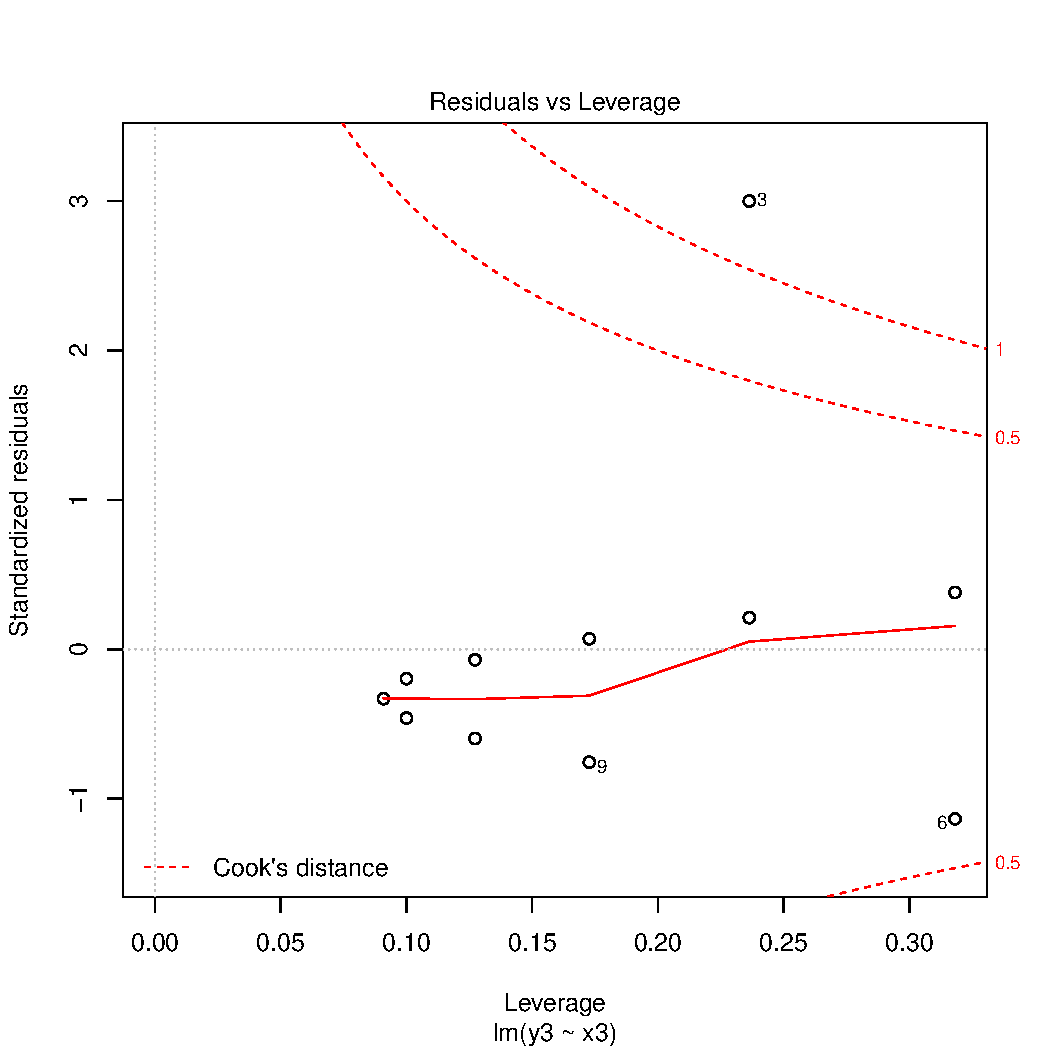
\includegraphics[width=\maxwidth]{figure/unnamed-chunk-14-1} 

\end{knitrout}

The Cook's D plot confirms that the third observation is an outlier, as it goes out of bound of the red lines denoting Cook's D $= 1$

\end{document}
